17. Расположите в кружочках числа от 1 до 10 так, чтобы для любых двух соседних чисел их сумма была равна сумме двух чисел, им противоположных (симметричных относительно центра окружности).
\begin{center}
\begin{figure}[ht!]
\center{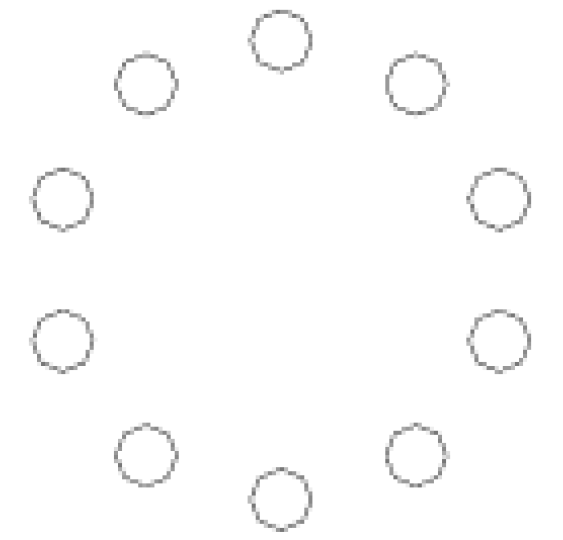
\includegraphics[scale=0.35]{3.png}}
\end{figure}
\end{center}

ewpage

oindent18. Расположите в кружочках числа от 11 до 20 так, чтобы для любых двух соседних чисел их сумма была равна сумме двух чисел, им противоположных (симметричных относительно центра окружности).
\begin{center}
\begin{figure}[ht!]
\center{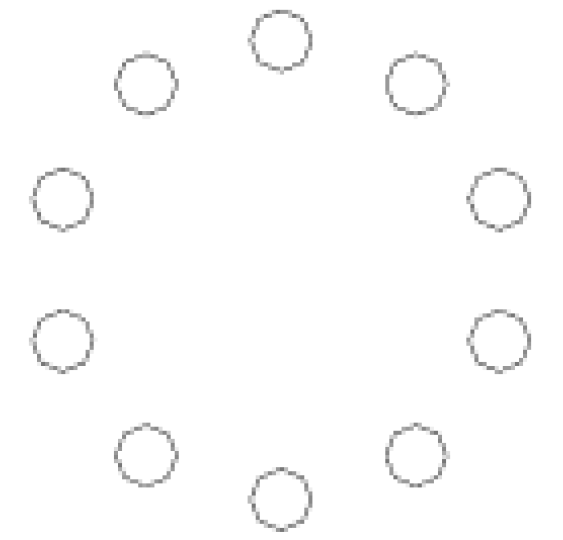
\includegraphics[scale=0.35]{33.png}}
\end{figure}
\end{center}
